\documentclass{article} % For LaTeX2e
\usepackage{nips15submit_e,times}
\usepackage{hyperref}
\usepackage{url}
\usepackage{graphicx}
\usepackage{mathtools}
\usepackage{float}
\usepackage[inline]{enumitem}
\usepackage{multirow}
\usepackage[toc,page]{appendix}
\usepackage{caption} 
\captionsetup[table]{skip=10pt}
\usepackage{cite}


%\documentstyle[nips14submit_09,times,art10]{article} % For LaTeX 2.09


\title{COMPGI19 Assignment 2 Report}

\author{
Kapileshwar Syamsundar
\And
Coauthor \\
Affiliation \\
Address \\
\texttt{email} \\
}

\newcommand{\fix}{\marginpar{FIX}}
\newcommand{\new}{\marginpar{NEW}}

\nipsfinalcopy % Uncomment for camera-ready version

\begin{document}

\maketitle

\section{Implementation of Perceptron Algorithm}
For this problem, we implemented a Perceptron trainer with the default setup; the results of our trainer and the precompiled trainer are shown in Table \ref{table:1_perf}.

\begin{table}[htb]
\centering
\caption{Classification performance for perceptron implementations}
\label{table:1_perf}
\begin{tabular}{l|l|l|}
\cline{2-3}
                                        & Our perceptron trainer & Precompiled perceptron trainer \\ \hline
\multicolumn{1}{|l|}{Average precision} & 0.5128644939965694     & 0.5262206148282098             \\ \hline
\multicolumn{1}{|l|}{Average recall}    & 0.6842105263157895     & 0.665903890160183              \\ \hline
\multicolumn{1}{|l|}{Average F1}        & 0.5862745098039216     & 0.5878787878787879             \\ \hline
\end{tabular}
\end{table}

The results show that our trainer has lower precision and higher recall than the precompiled trainer but, overall, has roughly the same harmonic mean of the two (F1).
\section{Implementation of Average Perceptron}

Our first implementation of the averaged perceptron involved keeping a running sum of the weights used for each prediction and then, after each instance and iteration, dividing the weights by the number of predictions made. However, this na�ve implementation is slow because every weight (even those that have not changed) is added to the sum of weights after every prediction and, in this domain, there are potentially many hundreds of thousands of features and respective weights. Therefore accessing and adding all of these weights for every training instance of every iteration is very inefficient.

Instead, we devised an alternate algorithm for accumulating the weights used for each prediction during training: for each prediction, only weights that are being changed (i.e. those associated with a candidate and the gold or predicted label) are added to the sum of weights, drastically reducing the number of weights accessed after each prediction. We achieve this by storing the last time each weight was modified so that when a weight is about to be changed, the duration of the current weight is known and can be multiplied by the weight to give the sum of that weight over the duration; this can then be added to the running sum of weights.

The results for our averaged perceptron with the default setup show it to be a lot better than the precompiled perceptron; these are shown in Table \ref{table:2_perf}.

\begin{table}[htb]
\centering
\caption{Classification performance for average perceptron implementations}
\label{table:2_perf}
\begin{tabular}{l|l|l|}
\cline{2-3}
                                        & Our average perceptron trainer & Precompiled average perceptron trainer \\ \hline
\multicolumn{1}{|l|}{Average precision} & 0.453125                       & 0.21044045676998369                    \\ \hline
\multicolumn{1}{|l|}{Average recall}    & 0.5308924485125858             & 0.5903890160183066                     \\ \hline
\multicolumn{1}{|l|}{Average F1}        & 0.48893572181243417            & 0.31028262176788934                    \\ \hline
\end{tabular}
\end{table}


\section{Feature Engineering and Evaluation}

In this section we outline and motivate potential feature templates for trigger and argument classification. Where possible, concrete training set examples are also provided. The best set of features (for both perceptron and Naive Bayes learning methods) are then presented.

Naive Bayes is a generative model and perceptron is discriminative.  Generative models account for the prior probability $p(x)$ of seeing a token. Maximising this model results in maximising $\log(p(y|x)) + \log(p(x))$. In text classification, we only care about finding the most likely label for a token, i.e. only maximising $p(y|x)$ and not $p(x)$. By optimising for both, we may sacrifice higher values for $p(y|x)$ to optimise for $p(x)$, giving us less accurate label predictions. However in the perceptron model, we only optimise for $p(y|x)$. This is why we expect the perceptron learning algorithm to perform better.

In choosing features for Naive Bayes, we consider that features are all independent and are weighted equally. This means that features should be tailored towards identifying specific labels instead of discriminating against the token being of a certain label. Further, choosing features that are similar will end up in maximising the prior probability instead of $p(y|x)$, resulting in poorer classification ability. We choose a subset of distinct features from the features outlined below that showed the best discriminative power.

Papers that provided inspiration for features have been referenced next to the feature name.

\subsection{Trigger features}

\subsubsection{Lexical}

\textbf{Stem of word.} Many events of the same label share a common stem. The transcription event is commonly associated with the token 'transcription', for instance. More generally in cases where we want to use the text of the token, we take the stem instead, allowing us to directly compare the meaning of the token. The suffix that we drop is an indication of its POS tag which we are given.

Our highest weighted feature for this class is having the stem ?transcript' for Transcription events. The feature also works well to discriminate against labels. For example, when the stem is ?inhibit?, a low weighting is given to the token being Positive regulation.

\emph{Increased interleukin 2 transcription in murine lymphocytes by ciprofloxacin}

\textbf{POS of word.} \cite{1} We expect words like conjunctions to be less likely to indicate events; typically we expect events to be verbs since they indicate an action. The highest weighted feature in this class is for tokens with POS tag CC (coordinating conjunction) to have label None. The lowest weighted feature is for tokens with POS tag VBN (verb, past participle) having label None, confirming our intuition that events tend to be verbs. 

Another example is labelling the token as Positive regulation if its POS is JJR (adjective, comparative). In our sentence below, the word \emph{stronger} is tagged as JJR.

\emph{Patients with diabetic nephropathy showed higher NF-kappaB binding activity in Electrophoretic Mobility Shift Assays and stronger immunohistological staining for activated NF-kappaBp65 than patients without renal complications}

We see that this feature performs strongest in determining whether or not a token is of label None.

\textbf{Capitalisation.} \cite{1} This feature counts the number of capital letters in the token. The immediate downside of this feature is that we also consider tokens that start at the beginning of a sentence which are capitalised regardless of their event classification. 

A highly weighted instance of this feature is assigning the token label Positive regulation when it has 2 capital letters, as in \emph{the word} in the sentence below.

\emph{fucked for now}

\subsubsection{Entity-based}

\textbf{Proteins in sentence.} We count the number of proteins in the sentence. Here our intuition is that having no proteins in the sentence makes it less likely that the sentence contains any event. We see that our highest weighted feature for this feature template is assigning a label of None to the current token if there are no proteins in the sentence giving evidence that our intuition is correct. However, this feature template doesn't discriminate well between events of type other than None.

\subsubsection{Syntax-based}

\textbf{Dependencies.} \cite{4} This class of features looks at the grammatical relations between words. Dependencies are an edge between two related words 'head' and 'mod' where 'head' refers to the source of the dependency and 'mod' is dependent on head. Experimentally we see that only considering dependencies as a feature doesn't perform well (this is a feature we implemented but chose not to select in the final set), so we also consider the POS and stem of the related dependency to our token. We think this is because whatever the explanation is. 

We consider features involving the mod/head, stem of the parent, dependency and POS. Here our token is the head. We consider these dependencies up to a depth of 3, meaning that if we have an edge between tokens A and B, we also consider the dependency between B and C and C and D (if they exist). An example of a well performing feature is assigning the Binding label to tokens where the edge to its associated token is prepAs (prepositional binding) and the associated token's POS is VBZ (verb, third person singular present). An example is given in Figure \ref{fig:dep_pos_mod}.

\subsubsection{Other}

\textbf{Context.} \cite{1} We capture the stems of immediately surrounding tokens. These tokens give us an understanding of the context in which the token is being used. We see in many cases that the previous token gives a clear indication of what the current token is. Our highest weighted feature for this class highly weights tokens being labelled as Transcription when the previous token is 'mRNA'. The previous word helps limit the events that the current token can be, so it works well in discriminating between all event labels. As a result, we see that we have highly negatively weighted features as well such as assigning the label Gene expression when the previous token is 'mRNA'.

\emph{There was no difference in the effects of AzaC versus AzadC , as both increased the IRF-4 mRNA level in CML-T1 cells as well ( data not shown )}

Features which look at the next token do not discriminate between the current token's possible labels as well as the previous token, but they help nonetheless. An example is assigning the label Positive regulation when the next token has stem 'chromosom'.

\subsubsection{Perceptron features}
\begin{itemize*}
\item Stem of word
\item POS of word
\item Number of capital letters in word
\item Prior word
\item Next word
\item Number of proteins in sentence
\item Level 1 dependency count
\item Level 2 dependency count
\item Level 3 dependency count
\item Level 1 dependency type and POS of mod
\item Level 2 dependency type and POS of mod
\item Level 3 dependency type and POS of mod
\item Level 1 dependency type and stem of mod
\item Level 2 dependency type and stem of mod
\item Level 3 dependency type and stem of mod
\item Level 1 dependency type and stem of head
\item Level 1 dependency type and POS of head
\end{itemize*}


\subsubsection{Naive-Bayes features}
\begin{itemize*}
\item Stem of word
\item Number of capital letters in word
\item Number of proteins in sentence
\item Level 1 dependency type and POS of mod
\end{itemize*}


\subsection{Argument features}

\subsubsection{Lexical}

\textbf{POS.} Part-of-speech features can provide semantic and contextual information related to the candidate and parent tokens of the data sets. For example, theme arguments generally have a part-of-speech value of 'NN', which can be used to differentiate theme arguments from cause and none types. Looking at the part-of-speech value for events can reveal information related to their child arguments as certain events are likely to have a specific part-of-speech related to them. The part-of-speech values can be combined to create unique pairs of them which can be used to map a specific argument classes to part-of-speech pairings in a one-to-many relationship. Refer to Figure \ref{fig:pos_candidate_parent} as an example.

\textbf{Value of word.} The word value of candidates and parents can be used as base measures to classify arguments as they will give a base relation between specific words and how they are related to arguments. Certain argument types are likely to relate to specific sets of words so creating features based on these values should provide a large amount of data for the classifier models to use. Conjunctions of word based features can also be used to create specific word pairs or sets that can be used to target argument types with higher precision.

\textbf{Stem.} Stem features provide a more generalised version of word features as the they group words related to a common theme. These can be very useful for determining what event the parent of the candidate relates to and in turn can reveal a significant amount of information related to the argument class of the candidate.

\textbf{Capitalised letters in candidate.} \cite{3} As certain candidates in the training set have capital letters in their names, we can use the set of capitalised letters to identify proteins more accurately and apply the information to classifying arguments.

\subsubsection{Entity-based}

\textbf{Candidate is a protein.} Upon inspection, many of the arguments of type cause and theme contain the protein tag under the mentions section. Therefore, we can filter out the arguments of type none by identifying whether the candidate is a protein or not. Refer to Figure \ref{fig:candidate_is_protein} as an example.

\textbf{Number of proteins.} Following on from the last feature, if there are no proteins in a sentence, then it is likely that the arguments in the sentence are of type none. As such, counting the number of proteins in the sentence can reveal the classification of the candidate.

\subsubsection{Syntax-based}

\textbf{McClosky dependency between candidate and parent.} \cite{1} In general, a specific type of McClosky dependency exists between an event and its arguments. Therefore, we can use these dependencies to map to specific argument types in order to classify a candidate. Refer to Figure \ref{fig:mc_dep_candidate_parent} as an example.

\textbf{Number of McClosky dependencies on candidate.} Counting the number of dependencies on the candidate can provide insight on what argument type it may be as arguments of a specific type can have more dependencies than others. In addition to this, it also recognises events which are also arguments effectively as they are likely to have many dependencies and relationships with other tokens in the data.

\textbf{Number of McClosky dependencies on parent.} Counting the number of dependencies on the parent can help classify which type of event it may relate to and therefore assist in classifying the candidate to a specific argument type.

\subsubsection{Other}

\textbf{Prior word.} As described in trigger features.

\textbf{Prior stem.} Creates a more general case for the prior word comparison by grouping words related to a specific theme.

\textbf{Prior POS.} For the same reason as the other prior techniques, creating pairs of parts-of-speech provide more contextual data to the classification process.

\textbf{Absolute token distance between candidate and parent.} \cite{2} From observing the training data, it can be seen that arguments are often located close to their parent token, meaning that bounds can be set to filter out arguments of type none. This value can be obtained as an absolute value or signed value to determine whether the candidate lies on the left or right side of it?s parent which can be used to obtain more positional information for specific arguments. Upon inspection of the training data, most distances above the value of 40 tended to be none-type arguments so the value was used as a cutoff point feature to classify none tokens.

\textbf{Candidate part-of-speech is 'NN' and is a protein.} A combination of part-of-speech and whether the candidate is a protein or not can be used to classify theme arguments specifically. From observation of the training set, there are an abundance of cases where a theme argument has the part-of-speech 'NN' and is also a protein. Refer to Figure \ref{candidate_nn_protein} as an example.

\subsubsection{Perceptron features}

\begin{itemize*}

\item Boolean check part-of-speech of candidate and parent are equivalent
\item Combination of the parts-of-speech of the candidate and parent
\item Combination of the stem of the candidate and parent
\item Combination of stem of parent and candidate protein tag check
\item Combination of if a capital letter exists in the candidate and protein tag check
\item Number of proteins in the sentence
\item Candidate protein tag check
\item Dependency from candidate to parent
\item Dependency from parent to candidate
\item Stem of prior word and candidate
\item Part-of-speech of prior word and candidate
\item Absolute distance between the candidate and parent in token units

\end{itemize*}

\subsubsection{Naive-Bayes features}

\begin{itemize*}

\item Combination of candidate part-of-speech and protein tag check
\item Boolean check if candidate and parent have equivalent parts-of-speech
\item Boolean check if a capital letter exists in the candidate and if it has a protein tag
\item McClosky dependency between the candidate and it?s parent
\item Boolean check if absolute distance between candidate and parent is less than 40
\item Boolean check if the number of proteins in the sentence is greater than zero
\item Prior part-of-speech check for candidate

\end{itemize*}

\subsection{Results}

\begin{table}[hbt]
\centering
\caption{Trigger classification results}
\label{perceptron_results_3}
\begin{tabular}{|l|l|l|l|l|}
\hline
Learning algorithm & Feature set used & Average precision & Average recall & Average F1 \\ \hline
Perceptron         & Perceptron       & 0.1940            & 0.8132         & 0.3133     \\ \hline
Naive Bayes        & Perceptron       & 0.0142            & 0.1323         & 0.0256     \\ \hline
Naive Bayes        & Naive Bayes      & 0.1609            & 0.7500         & 0.2650     \\ \hline
\end{tabular}
\end{table}

First we implemented lexical features, yielding an average F1 score of 0.1237. Adding entity features increased the score to 0.1735. Syntax features increased the score by a considerable amount to 0.2540. Finally including all other features raised the score to 0.3133. 

\begin{table}[hbt]
\centering
\caption{Argument classification results}
\label{argument_results_3}
\begin{tabular}{|l|l|l|l|l|}
\hline
Learning algorithm & Feature set used & Average precision & Average recall & Average F1 \\ \hline
Perceptron         & Perceptron       & 0.07338           & 0.8675         & 0.1353     \\ \hline
Naive Bayes        & Perceptron       & 0.01311           & 0.9066         & 0.02585    \\ \hline
Naive              & Naive Bayes      & 0.06565           & 0.6635         & 0.1195     \\ \hline
\end{tabular}
\end{table}

As additional features were applied to the models, the improvements to the scores were recorded to provide insight as to which groups of features provided the largest overall benefit. For the perceptron model, the lexical features alone provided an average F1 score of 0.0375 showing that alone they did not provide accurate classifications. However, adding entity features improves the score to 0.0494 showing that these features work well in conjunction with each other. Adding syntactic features using the McClosky dependencies between words improves the score further by to 0.0628 and adding prior word features on top that pushes the score to 0.0985. Finally, adding positional features provides the final score of 0.1353.

For the Naive Bayes model, using only the lexical features provides an F1 score of 0.12 but it does not classify any cause statements whatsoever. Therefore, additional features were added in an attempt to classify cause at the expense of the F1 score. Adding entity features didn?t provide any assistance in classifying cause and also didn?t alter the F1 score. However, adding syntactic and positional features allowed for the model to classify theme arguments and only changed the F1 score to 0.119.

\section{Joint Perceptron}

\subsection{Unconstrained joint model}
The joint classifier classifies arguments and triggers together. This means that the output of the classifier's prediction function is a tuple that contains the best choice of labels (as dictated by the weights from training) for the trigger and its arguments. This can be represented as a sum of the score for the event trigger and the scores for its arguments. As the score for the triggers and arguments is dependent on their labels, maximising the overall score corresponds to finding the best labels. 

Because the unconstrained model is such that the label assigned to a trigger is independent to the labels assigned to its arguments, maximising the total score is equivalent to individually maximising the trigger and argument scores. So given a candidate, the relevant feature vector, weights and a set of possible labels for the candidate, we can define a generic argmax routine to return the most likely label. The pseudo code for such an argmax algorithm is shown below:

\begin{verbatim}
argmax(labels, candidate, weights, feat):
  scores = []
  for (elem in labels):
   featureVector = feat(candidate, elem) // create feature Vector
   score = dot(weights, featureVector)       
   scores.append((score, elem))

   // return the label of the score with highest score value
   return maxBy(scores.elem).label 
\end{verbatim}

\subsection{Constrained joint model}
As with the unconstrained version of the joint model, the scores are calculated for each trigger label and then for the argument labels for each argument and these are summed to give the overall scores for the joint structure.

For the constrained version of the joint model, the score for each trigger label is calculated and stored, rather than just storing the score of the label that maximises the score for the trigger. Then, for each trigger label, the argument labels are predicted with the required constraints in place.

Two of the constraints, 'A trigger can only have arguments if its own label is not NONE' and 'Only regulation events can have CAUSE arguments', are enforced by removing illegal argument labels from the set of possible argument labels. For example, when the trigger label is 'None', the arguments labels 'Theme' and 'Cause' are removed from the set of legal argument labels. These legal argument labels are the ones used in calculate the argmax of the arguments.

The final constraint, 'A trigger with a label other than NONE must have at least one THEME', is implemented by, for each argument, calculating the score of it being 'Theme' plus the maximum score of the other arguments given the available labels. The maximum score of these is then added to the score of the trigger and the trigger and argument labels that give the maximum of these trigger-argument combined scores is returned as the argmax for this joint constrained model.

This method of implementing the constraints is a lot more efficient than calculating all possible combinations of arguments and their scores for each label and then filtering out those that violate the constraints before returning the label combination with the maximum score.

\begin{verbatim}
argmax(triggerLabels, argLabels, x):
  
  for (tlabel in triggerLabels):
    triggerScore(tlabel) = score(x, tlabel)
    if (tlabel is "None") {
      currentArgLabels = argLabels - "Theme" - "Cause"
    }
    else if (tlabel is not a regulation event label) {
      currentArgLabels = argLabels - "Cause"
    }
    else {
      currentArgLabels = argLabels
    }
  
  for (arg in x.arguments):
    argScore(arg) = score(arg, "Theme") + ...
        sum(maxScore(x.arguments != arg))
    totalScore(tlabel) = triggerScore(tlabel) + max(argScore)
    return max(totalScore).labels
\end{verbatim}

\section{Implementation and Evaluation for Problem 4}

Using the default split of 80\% training data and 20\% development data from 500 documents, we trained the per-task models from Problem 3 and the two joint models from Problem 4 over the default number of iterations, 10.

\begin{table}[htb]
\centering
\caption{Performance of models}
\label{table:all_perf}
\resizebox{\textwidth}{!}{%
\begin{tabular}{|c|l|l|l|l|}
\hline
\multicolumn{1}{|l|}{Candidate} & Metric            & Per-task Models & Unconstrained Joint Model & Constrained Joint Model \\ \hline
\multirow{3}{*}{Trigger}        & Average precision & 0.1940          & 0.1806                    & 0.2729                  \\ \cline{2-5} 
                                & Average recall    & 0.8132          & 0.8003                    & 0.7691                  \\ \cline{2-5} 
                                & Average F1        & 0.3133          & 0.2947                    & 0.4029                  \\ \hline
\multirow{3}{*}{Argument}       & Average precision & 0.07338         & 0.1362                    & 0.1864                  \\ \cline{2-5} 
                                & Average recall    & 0.8675          & 0.6330                    & 0.3880                  \\ \cline{2-5} 
                                & Average F1        & 0.1353          & 0.2242                    & 0.2518                  \\ \hline
\end{tabular}
}
\end{table}
The average F1 results in Table \ref{table:all_perf}  show that the joint models are a lot better at predicting the argument labels than the per-task model, with the constrained joint model being the best. Although the recall of argument labels is decreased for both joint models, the precision is increased, resulting in a higher average harmonic mean between the two metrics. However, it is the opposite for trigger classification: the joint models perform worse than the per-task model, with the constrained joint model performing the worst. The unconstrained joint model does have a higher recall than the per-task model for triggers but the decrease in precision for both models results in a lower average harmonic mean.
It is likely that the reason for the constrained joint model having the highest average precision for arguments is that the set of labels is reduced for most argument candidates as a result of the constraints.

\section{Error Analysis}
\subsection{Best model}
Overall we found our best model to be the joint constrained model, trained on the perceptron learning algorithm. The performance metrics we valued the highest when choosing our best model were precision and harmonic mean. While recall scores indicated a measure of completeness (quantity), we opted for precision?s measure of exactness (quality) as a more relevant performance indicator.

\subsection{Types of errors}
With an average precision of 0.273, all labels suffered from errors in classification. The event label with the least misclassifications was phosphorylation while the model struggled with precision for regulation events the most. It was found that the most common types of errors (across all types of triggers) were mislabelling candidate triggers to be none. The following sentence shows an instance of this.

?Activation and expression of the nuclear factors of activated T cells, NFATp and NFATc, in human natural killer cells: regulation upon CD16 ligand binding.?

For argument classification, average precision was 0.187. As with trigger classification, it was found that the main error was misclassifying candidate arguments to be of type none. An example instance of when this happened is shown below.

?Both nuclear run-on and actinomycin D pulse experiments strongly indicate that HU regulates c-jun mRNA expression by increasing the rate of synthesis as well as stabilizing the c-jun mRNA.?

The frequency of these types of errors can be inferred from tables \ref{table:trigs_results} and \ref{table:args_results}, where the columns represent the predicted label and the rows represent the true label.

\begin{table}[htb]
\centering
\caption{Predictions vs true labels for event triggers}
\label{table:trigs_results}
\resizebox{\textwidth}{!}{%
\begin{tabular}{|l|l|l|l|l|l|l|l|l|l|l|}
\hline
Gold | Prediction   & Phosphorylation & Negative regulation & Regulation & Protein catabolism & Binding & Positive regulation & Localization & Transcription & None & Gene expression \\ \hline
Phosphorylation     & 18              & 0                   & 0          & 0                  & 0       & 0                   & 0            & 0             & 2    & 0               \\ \hline
Negative regulation & 0               & 47                  & 3          & 0                  & 0       & 6                   & 0            & 1             & 10   & 5               \\ \hline
Regulation          & 0               & 0                   & 63         & 0                  & 0       & 11                  & 1            & 0             & 13   & 3               \\ \hline
Protein catabolism  & 0               & 0                   & 0          & 10                 & 0       & 0                   & 0            & 0             & 5    & 0               \\ \hline
Binding             & 0               & 1                   & 1          & 0                  & 54      & 6                   & 0            & 0             & 11   & 7               \\ \hline
Positive regulation & 0               & 1                   & 10         & 0                  & 0       & 172                 & 0            & 0             & 32   & 13              \\ \hline
Localization        & 0               & 0                   & 0          & 0                  & 0       & 0                   & 25           & 0             & 0    & 6               \\ \hline
Transcription       & 0               & 0                   & 1          & 0                  & 0       & 0                   & 1            & 38            & 5    & 13              \\ \hline
None                & 12              & 83                  & 279        & 11                 & 174     & 564                 & 31           & 89            & 5649 & 241             \\ \hline
Gene expression     & 0               & 0                   & 0          & 0                  & 0       & 5                   & 1            & 0             & 4    & 166             \\ \hline
\end{tabular}
}
\end{table}

\begin{table}[htb]
\centering
\caption{Predictions vs true labels for argument triggers}
\label{table:args_results}
\begin{tabular}{|l|l|l|l|}
\hline
Gold | Prediction & None & Theme & Cause \\ \hline
None & 84070 & 1763 & 3 \\ \hline
Theme & 554 & 407 & 0 \\ \hline
Cause & 77 & 11 & 0 \\ \hline
\end{tabular}
\end{table}

\subsection{Errors it helps to prevent}
In the joint models, arguments and triggers are predicted together and so classification occurs together. This idea is very useful for argument extraction as an argument is defined over multiple words (source trigger and the argument candidate itself).

So the types of error that joint models help prevent are mainly applicable to arguments where prior knowledge of the trigger label influences the labels for its corresponding arguments. For example, if it is known that the trigger is regulation, then the arguments for such a trigger can be limited to only be of label cause. 

As a result, even if the trained weights predict an illegal label, through constraints we can force classifications to a label (potentially the correct one) of a lower score.


\subsection{Unresolved errors}
Using joint model, we can resolve further errors with argument features by enforcing further constraints and heuristics from studying the dataset that target specific trigger labels and limit the range of legal possibilities for given argument candidates. This would primarily help resolve errors where candidates with true labels that are not none are mislabelled as other non ?none? labels. However, as observed by the error analysis, these instances are quite rare. 

Although the constraints lower the number of possible label combinations to predict, it does not address the problem of candidates misclassified as none. This problem lies with the features chosen. The current features do not help to strongly discriminate between identifying candidates with label none against other specific labels. This is why the majority of the incorrectly predicted candidates are labelled as none. In the case of the label Cause, it is always predicted as none Engineering features that capture information more relevant to specific labels (as opposed to those that are more generic to any label) are how such errors can be resolved.

Another way to potentially resolve errors could be to change from a joint model to a pipeline one. In this pipeline model, triggers could be predicted labels first and then these predictions incorporated when predicting arguments. This means feature templates for arguments could access predicted parent token labels. The pipeline model would still effectively be a joint model but the constraints are implemented on a lower level instead, where they can be of a more specific and complex nature.



\newpage
\begin{appendices}
\section{Examples of trigger features}

\begin{figure}[H]
  \caption{Dependency type of POS of mod}
  \centering
    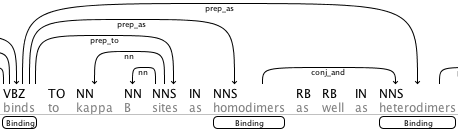
\includegraphics[width=0.75\textwidth]{images/trig_1.png}
      \label{fig:dep_pos_mod}
\end{figure}

\section{Examples of argument features}

\begin{figure}[H]
  \caption{POS of candidate and parent}
  \centering
    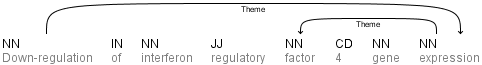
\includegraphics[width=0.75\textwidth]{images/arg_1.png}
      \label{fig:pos_candidate_parent}
\end{figure}

\begin{figure}[H]
  \caption{Candidate is a protein}
  \centering
    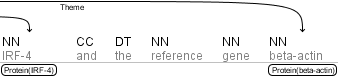
\includegraphics[width=0.75\textwidth]{images/arg_4.png}
      \label{fig:candidate_is_protein}
\end{figure}

\begin{figure}[H]
  \caption{McClosky dependency between candidate and parent}
  \centering
    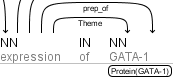
\includegraphics[width=0.30\textwidth]{images/arg_7.png}
      \label{fig:mc_dep_candidate_parent}
\end{figure}

\begin{figure}[H]
  \caption{Candidate POS is NN and is a protein}
  \centering
    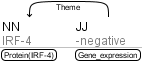
\includegraphics[width=0.30\textwidth]{images/arg_10.png}
      \label{candidate_nn_protein}
\end{figure}

\end{appendices}

\bibliography{references}{}
\bibliographystyle{plain}

\end{document}